\begin{tikzpicture}[x=0.75pt,y=0.75pt,yscale=-0.7,xscale=0.7]
    %uncomment if require: \path (0,523); %set diagram left start at 0, and has height of 523
    
    %Shape: Rectangle [id:dp7131803617577668] 
    \draw  [draw opacity=0][fill={rgb, 255:red, 74; green, 144; blue, 226 }  ,fill opacity=0.1 ] (196,288) -- (223.83,288) -- (223.83,473.85) -- (196,473.85) -- cycle ;
    %Straight Lines [id:da7598722594677334] 
    \draw    (266,474) -- (486.83,474) ;
    \draw [shift={(488.83,474)}, rotate = 180] [fill={rgb, 255:red, 0; green, 0; blue, 0 }  ][line width=0.08]  [draw opacity=0] (12,-3) -- (0,0) -- (12,3) -- cycle    ;
    %Image [id:dp8241642666901281] 
    \draw (360.92,369.08) node  {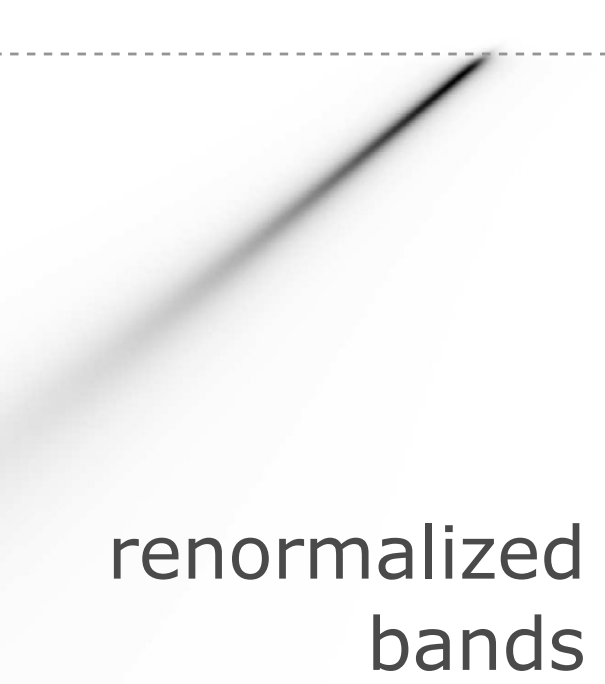
\includegraphics[width=100.71pt,height=100.71pt]{plot/arpes-spectrum-example-1.PNG}};
    %Straight Lines [id:da6586111996921291] 
    \draw    (266,474) -- (266,247.85) ;
    \draw [shift={(266,245.85)}, rotate = 90] [fill={rgb, 255:red, 0; green, 0; blue, 0 }  ][line width=0.08]  [draw opacity=0] (12,-3) -- (0,0) -- (12,3) -- cycle    ;
    %Straight Lines [id:da35625894168032457] 
    \draw    (224,474) -- (224,247.85) ;
    \draw [shift={(224,245.85)}, rotate = 90] [fill={rgb, 255:red, 0; green, 0; blue, 0 }  ][line width=0.08]  [draw opacity=0] (12,-3) -- (0,0) -- (12,3) -- cycle    ;
    %Straight Lines [id:da943265616635429] 
    \draw [color={rgb, 255:red, 74; green, 144; blue, 226 }  ,draw opacity=1 ]   (196,288) -- (223.83,288) ;
    %Straight Lines [id:da6139331520486002] 
    \draw [color={rgb, 255:red, 74; green, 144; blue, 226 }  ,draw opacity=1 ]   (196,288) -- (196.17,474) ;
    %Straight Lines [id:da8048536335889904] 
    \draw [color={rgb, 255:red, 74; green, 144; blue, 226 }  ,draw opacity=1 ]   (223.83,257.85) -- (223.83,288) ;
    %Straight Lines [id:da1675470318517831] 
    \draw  [dash pattern={on 0.84pt off 2.51pt}]  (223.83,288) -- (265.83,288) ;
    %Straight Lines [id:da12246512878622995] 
    \draw  [dash pattern={on 0.84pt off 2.51pt}]  (459.83,288) -- (501.83,288) ;
    %Straight Lines [id:da8543910261314052] 
    \draw    (223.83,473.85) -- (156.67,473.85) ;
    \draw [shift={(154.67,473.85)}, rotate = 360] [fill={rgb, 255:red, 0; green, 0; blue, 0 }  ][line width=0.08]  [draw opacity=0] (12,-3) -- (0,0) -- (12,3) -- cycle    ;
    %Straight Lines [id:da9955938989460331] 
    \draw    (266,195.85) -- (486.83,195.85) ;
    \draw [shift={(488.83,195.85)}, rotate = 180] [fill={rgb, 255:red, 0; green, 0; blue, 0 }  ][line width=0.08]  [draw opacity=0] (12,-3) -- (0,0) -- (12,3) -- cycle    ;
    %Straight Lines [id:da18702951363365972] 
    \draw    (266,195.85) -- (266,125.92) ;
    \draw [shift={(266,123.92)}, rotate = 90] [fill={rgb, 255:red, 0; green, 0; blue, 0 }  ][line width=0.08]  [draw opacity=0] (12,-3) -- (0,0) -- (12,3) -- cycle    ;
    %Straight Lines [id:da2056417168381537] 
    \draw  [dash pattern={on 0.84pt off 2.51pt}]  (419,125.31) -- (419,473.52) ;
    %Shape: Polygon Curved [id:ds2789435512931895] 
    \draw  [color={rgb, 255:red, 74; green, 144; blue, 226 }  ,draw opacity=1 ][fill={rgb, 255:red, 74; green, 144; blue, 226 }  ,fill opacity=0.1 ] (265.85,155.02) .. controls (332.6,156.3) and (406.6,152.55) .. (418.6,162.05) .. controls (419.13,175.27) and (418.38,162.27) .. (419.13,188.77) .. controls (429.13,194.02) and (434.13,194.77) .. (453.13,195.77) .. controls (406.13,195.77) and (360.38,195.77) .. (266,195.85) .. controls (266.1,155.52) and (266.35,195.77) .. (265.85,155.02) -- cycle ;
    %Straight Lines [id:da08475461712586241] 
    \draw  [dash pattern={on 0.84pt off 2.51pt}]  (265.85,155.02) -- (419.88,155.02) ;
    
    % Text Node
    \draw (490.83,474) node [anchor=west] [inner sep=0.75pt]    {$k$};
    % Text Node
    \draw (266,242.85) node [anchor=south] [inner sep=0.75pt]    {$\omega $};
    % Text Node
    \draw (224.19,242.85) node [anchor=south] [inner sep=0.75pt]  [rotate=-358.35]  {$\omega $};
    % Text Node
    \draw (503.83,288) node [anchor=west] [inner sep=0.75pt]    {$\varepsilon _{\text{F}}$};
    % Text Node
    \draw (152.67,473.85) node [anchor=east] [inner sep=0.75pt]   [align=left] {$\displaystyle n( \omega ) /D( \omega )$};
    % Text Node
    \draw (490.83,195.85) node [anchor=west] [inner sep=0.75pt]    {$k$};
    % Text Node
    \draw (266,120.92) node [anchor=south] [inner sep=0.75pt]   [align=left] {$\displaystyle n_{k}$};
    % Text Node
    \draw (419,476.52) node [anchor=north] [inner sep=0.75pt]    {$p_{\text{F}}$};
    
    
    \end{tikzpicture}
    